\documentclass{beamer}
\usetheme{CambridgeUS}
\usefonttheme{structurebold}
\usecolortheme{seahorse}
\setbeamertemplate{caption}[numbered]
\setbeamerfont{caption}{size=\footnotesize}
% following suppresses navigation symbols
\setbeamertemplate{navigation symbols}{}
% following gets page numbers to show up
\setbeamertemplate{footline}[frame number]{}
\newtheorem{hypothesis}{Hypothesis}
\newtheorem{question}{Question}
\author{Jana E. Beck}
\title{Quantifying Diabetes}
\subtitle{Lessons learned from 100,000+ blood glucose readings}
\date{May 8, 2012}
\usepackage{color}
\usepackage{graphicx}
\usepackage{multirow}
\usepackage{multicol}
\usepackage{hyperref}
\hypersetup{colorlinks,urlcolor=blue,linkcolor=black}
\begin{document}

\begin{frame}
\maketitle
\end{frame}

\section{Background}

\begin{frame}
  \frametitle{Type 1 Diabetes}

  \begin{itemize}
  \item an auto-immune disease\\
    = the body's immune system attacks and kills the insulin-producing $\beta$-cells in the
    pancreas
  \item very little to no endogenous insulin production\\
    = dependent on synthetic insulin
  \item insulin dosing \textbf{is not easy!}
    \begin{itemize}
    \item basal insulin
    \item bolus insulin\\
      = matched to carbohydrates consumed, roughly
    \end{itemize}
  \end{itemize}

\end{frame}

\begin{frame}
  \frametitle{Continuous Glucose Monitoring}


    \begin{center}
      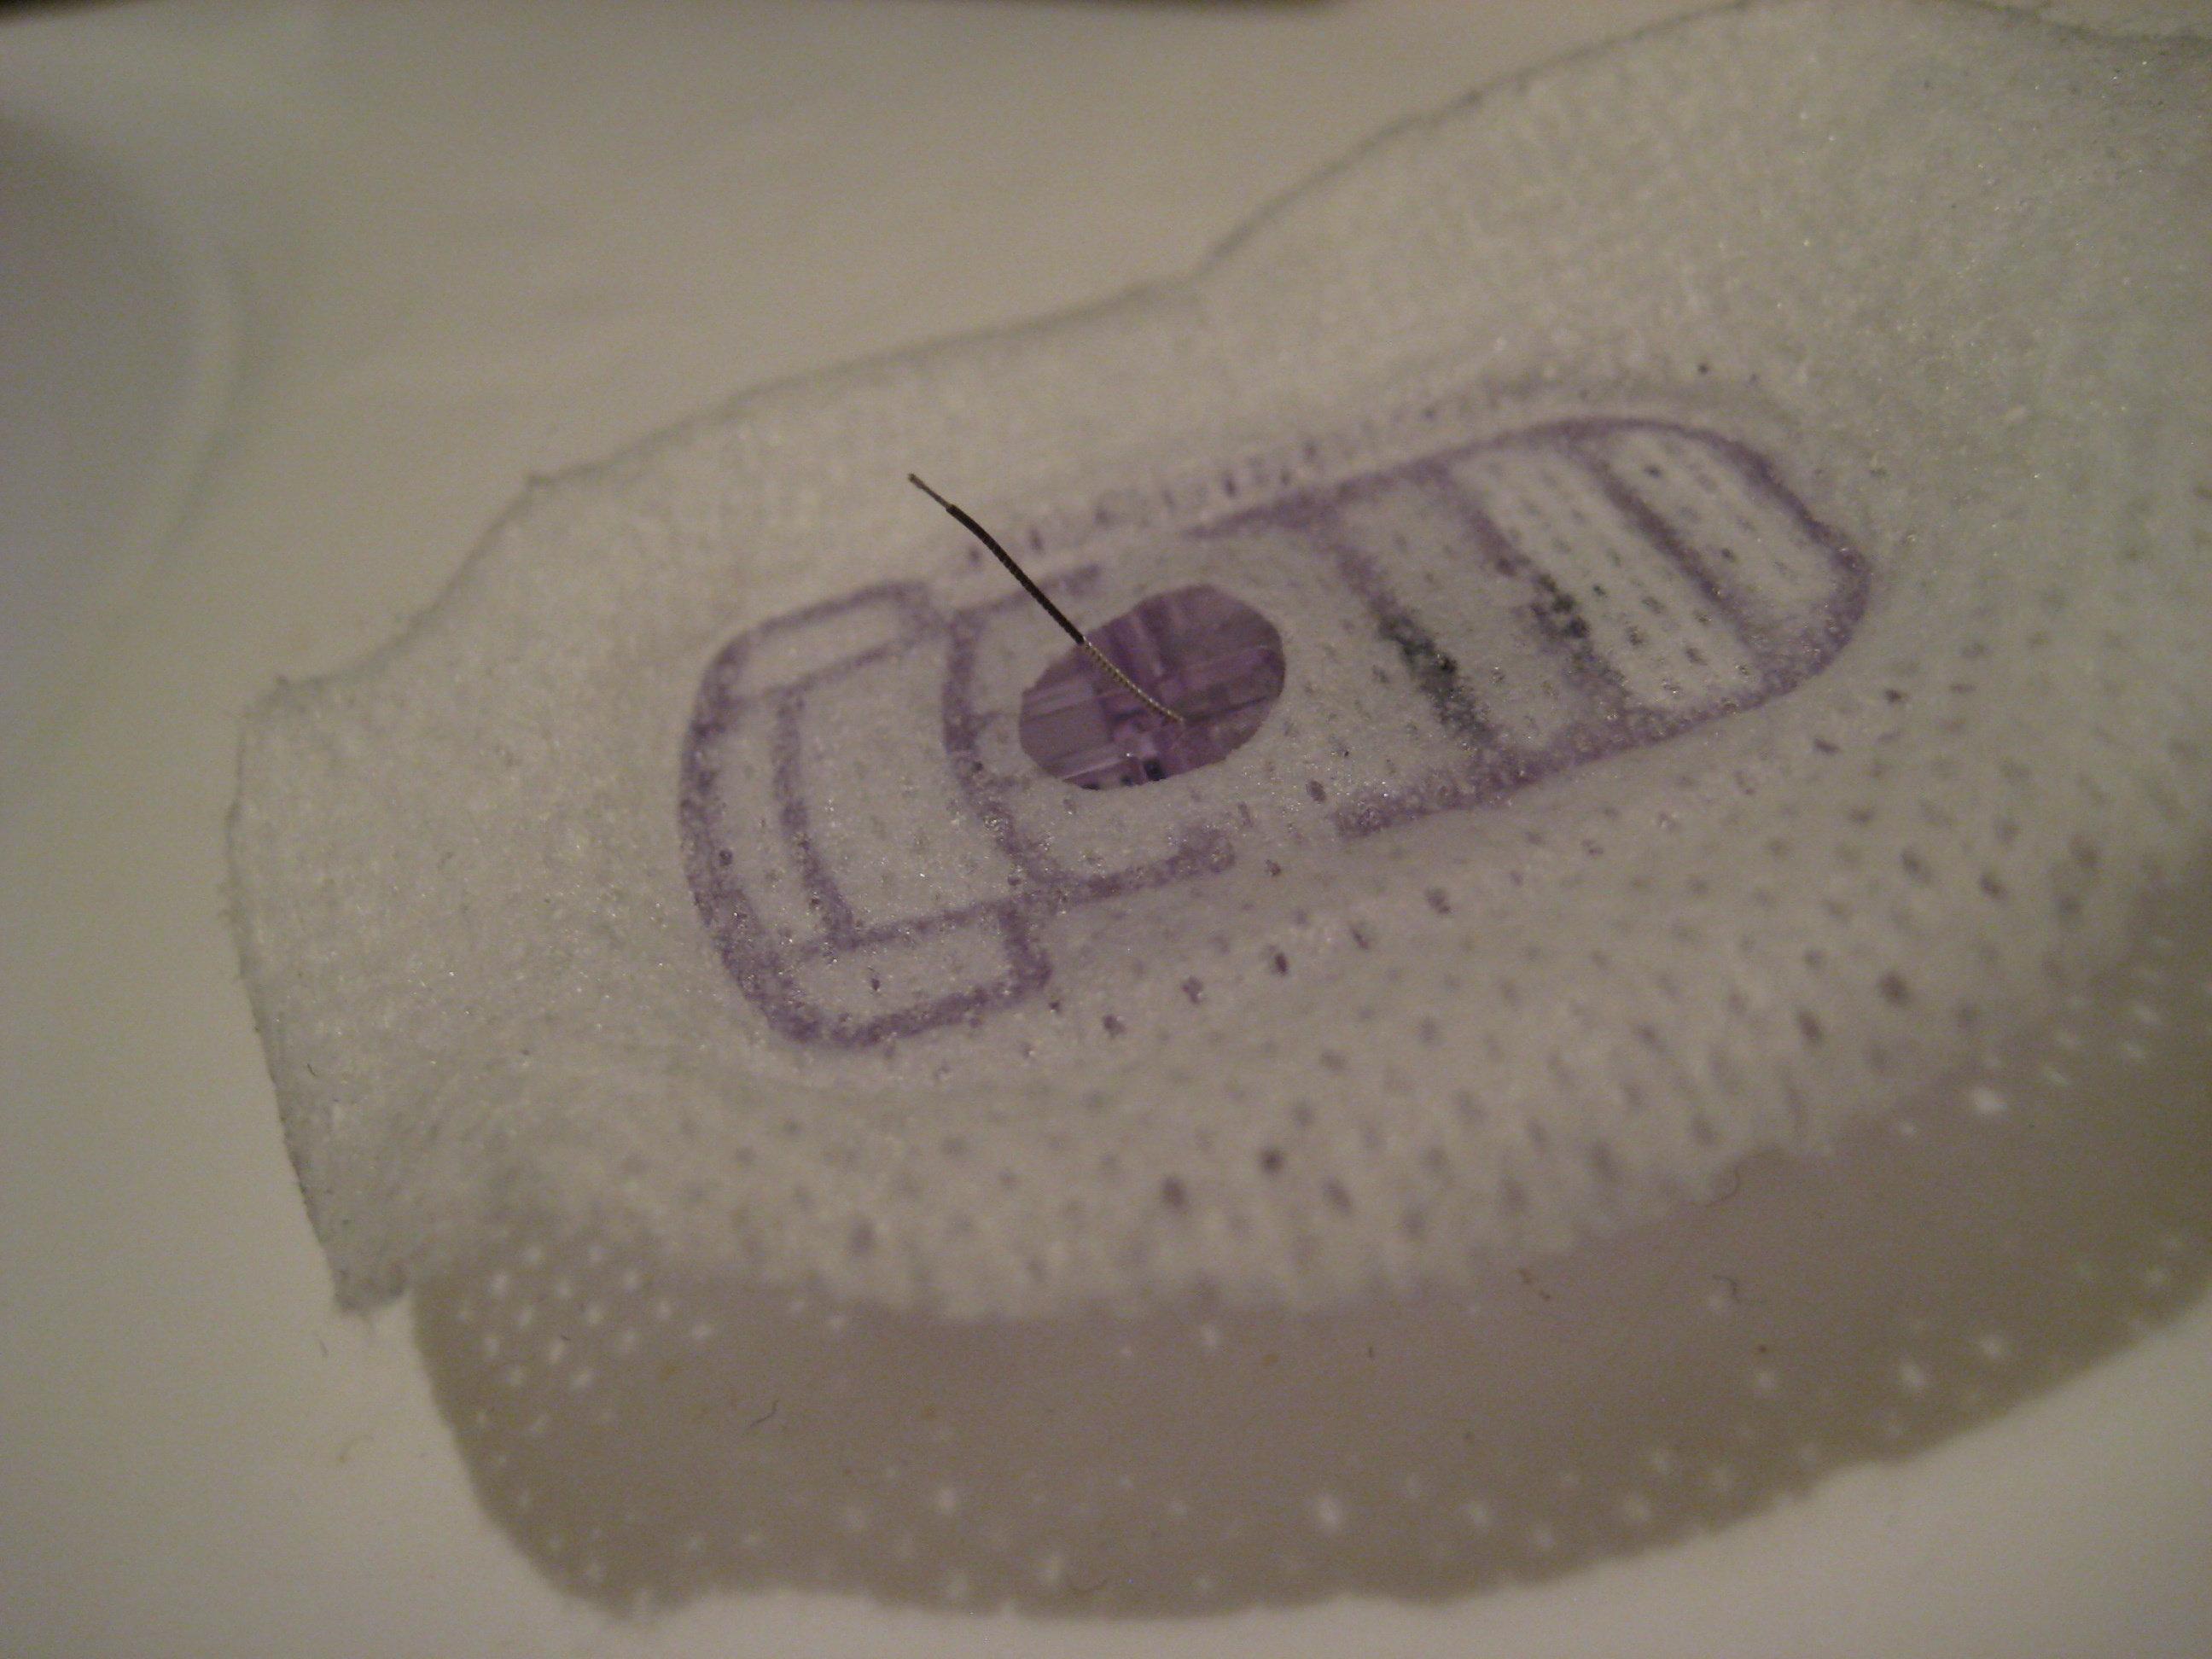
\includegraphics[width=.3\linewidth]{dexcom1.jpg}
      \hskip .05in
      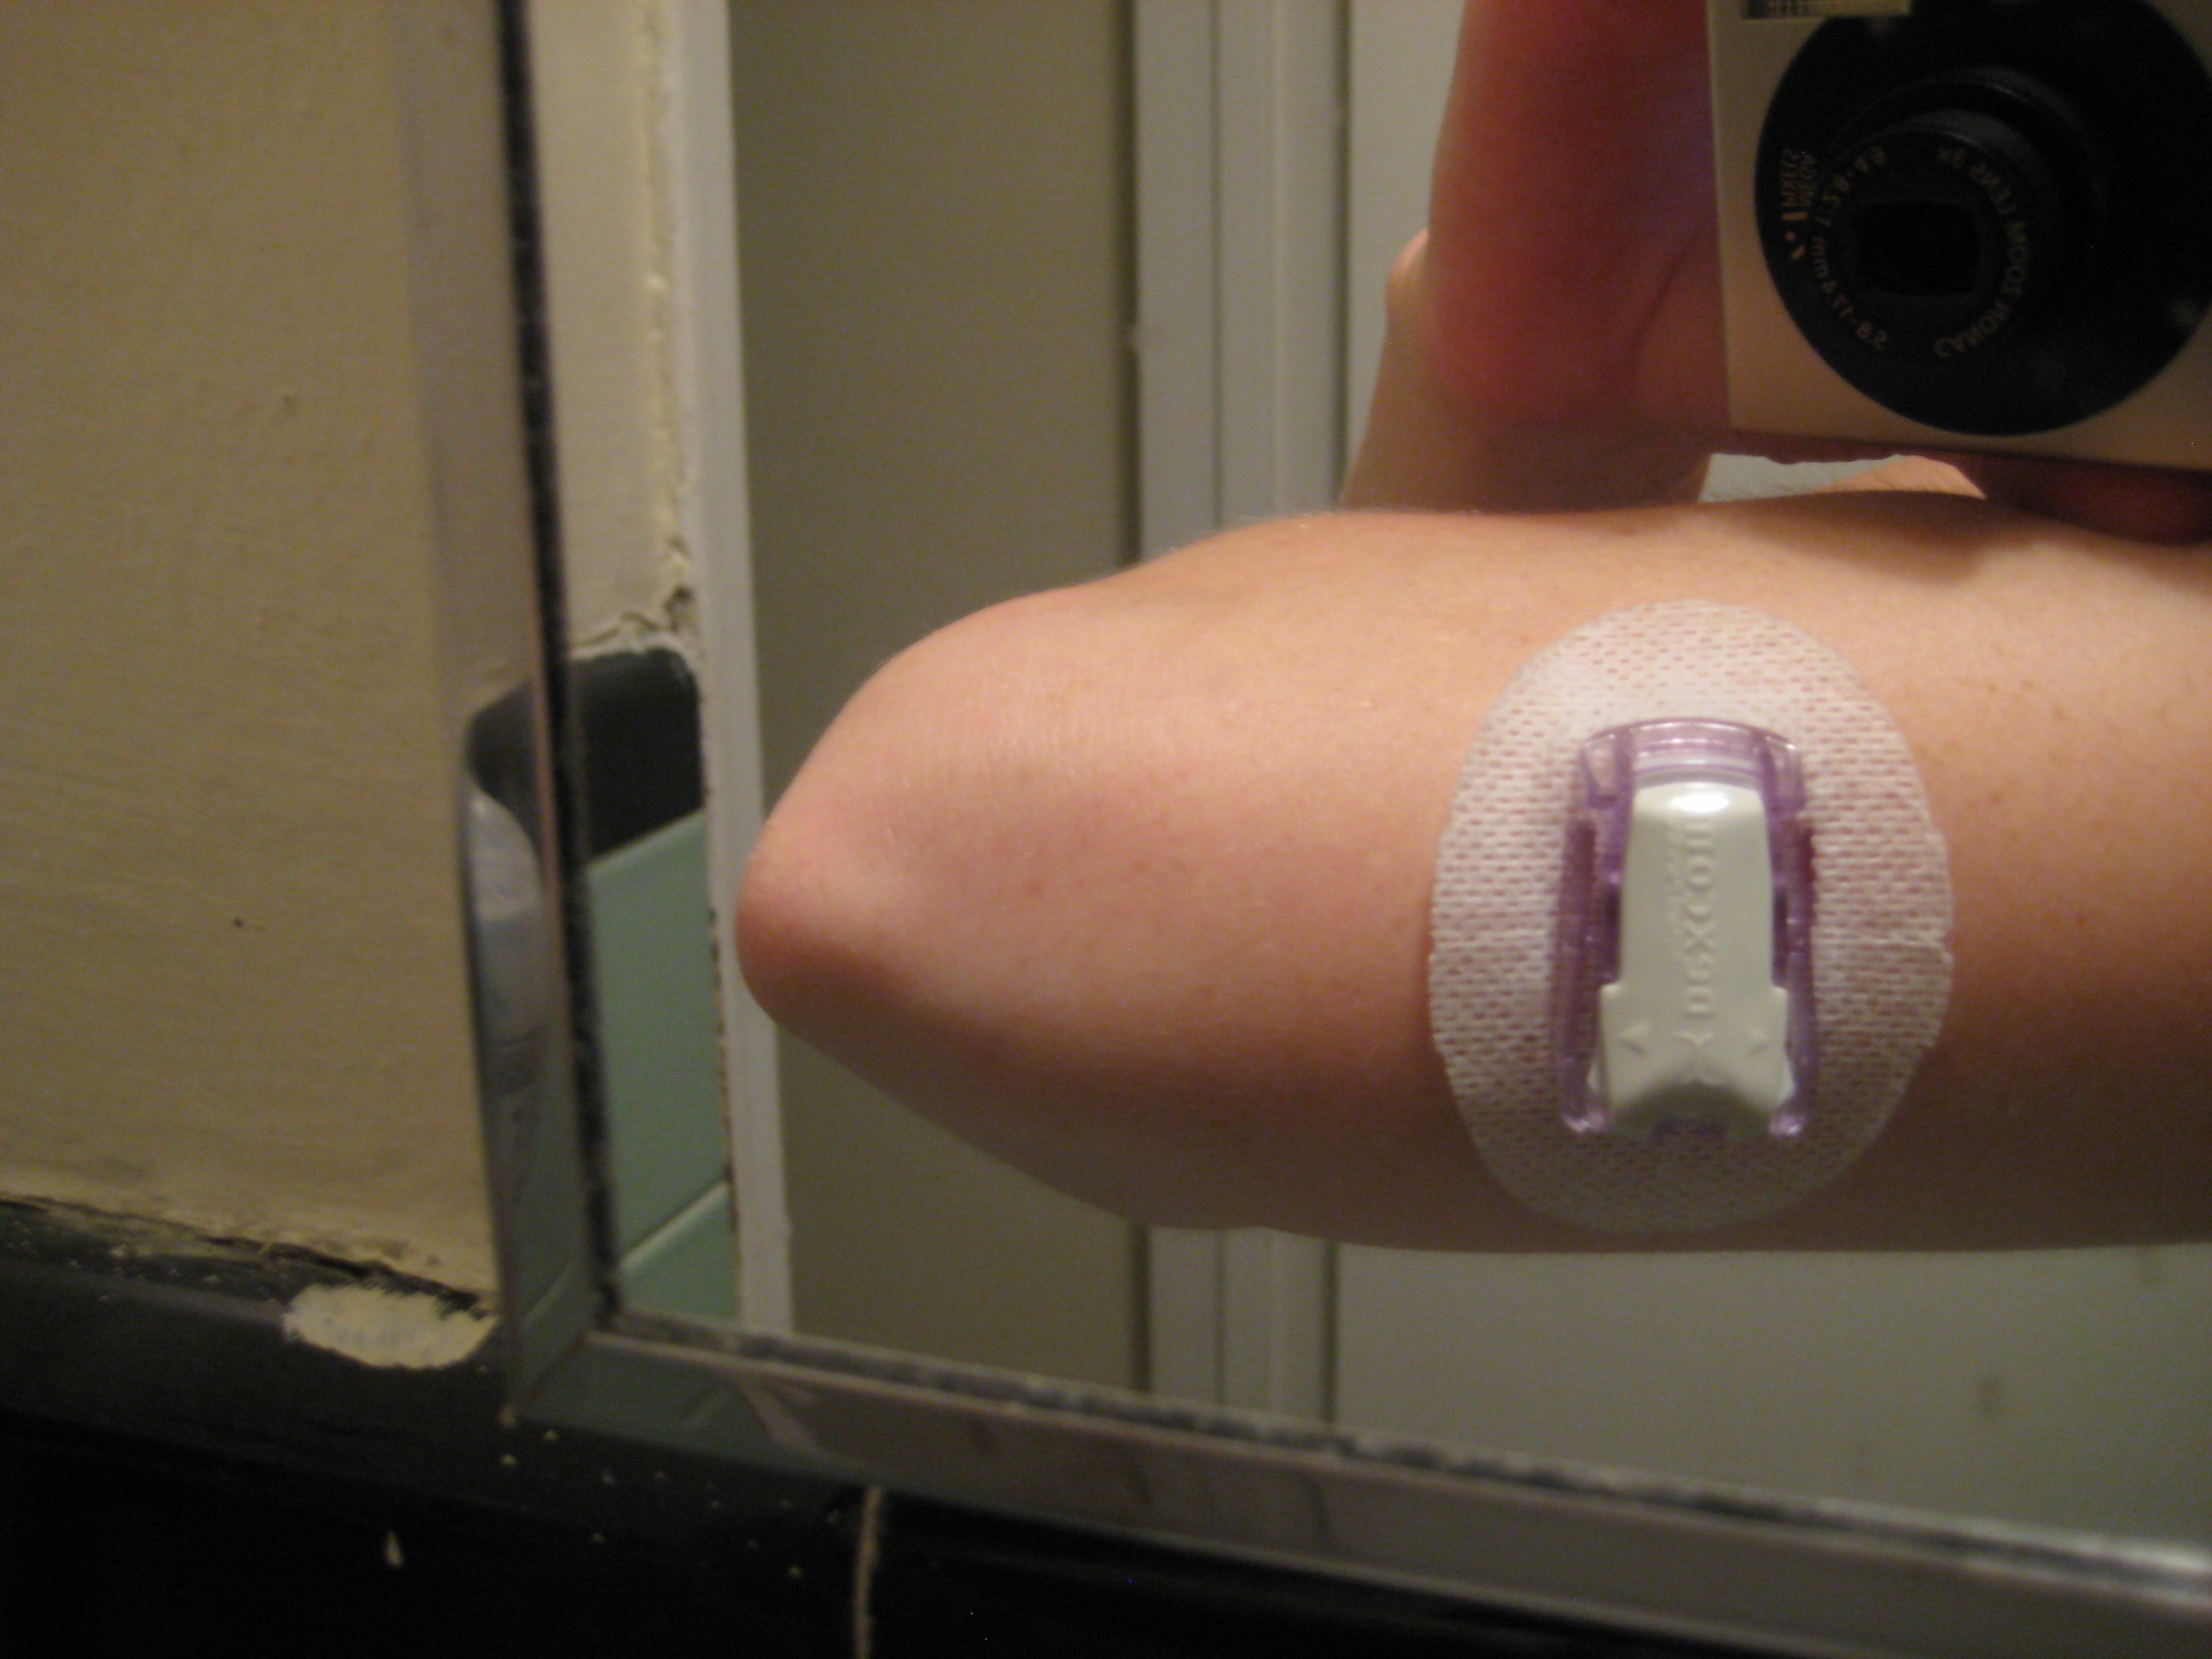
\includegraphics[width=.3\linewidth]{dexcom2.jpg}
      \hskip .05in
      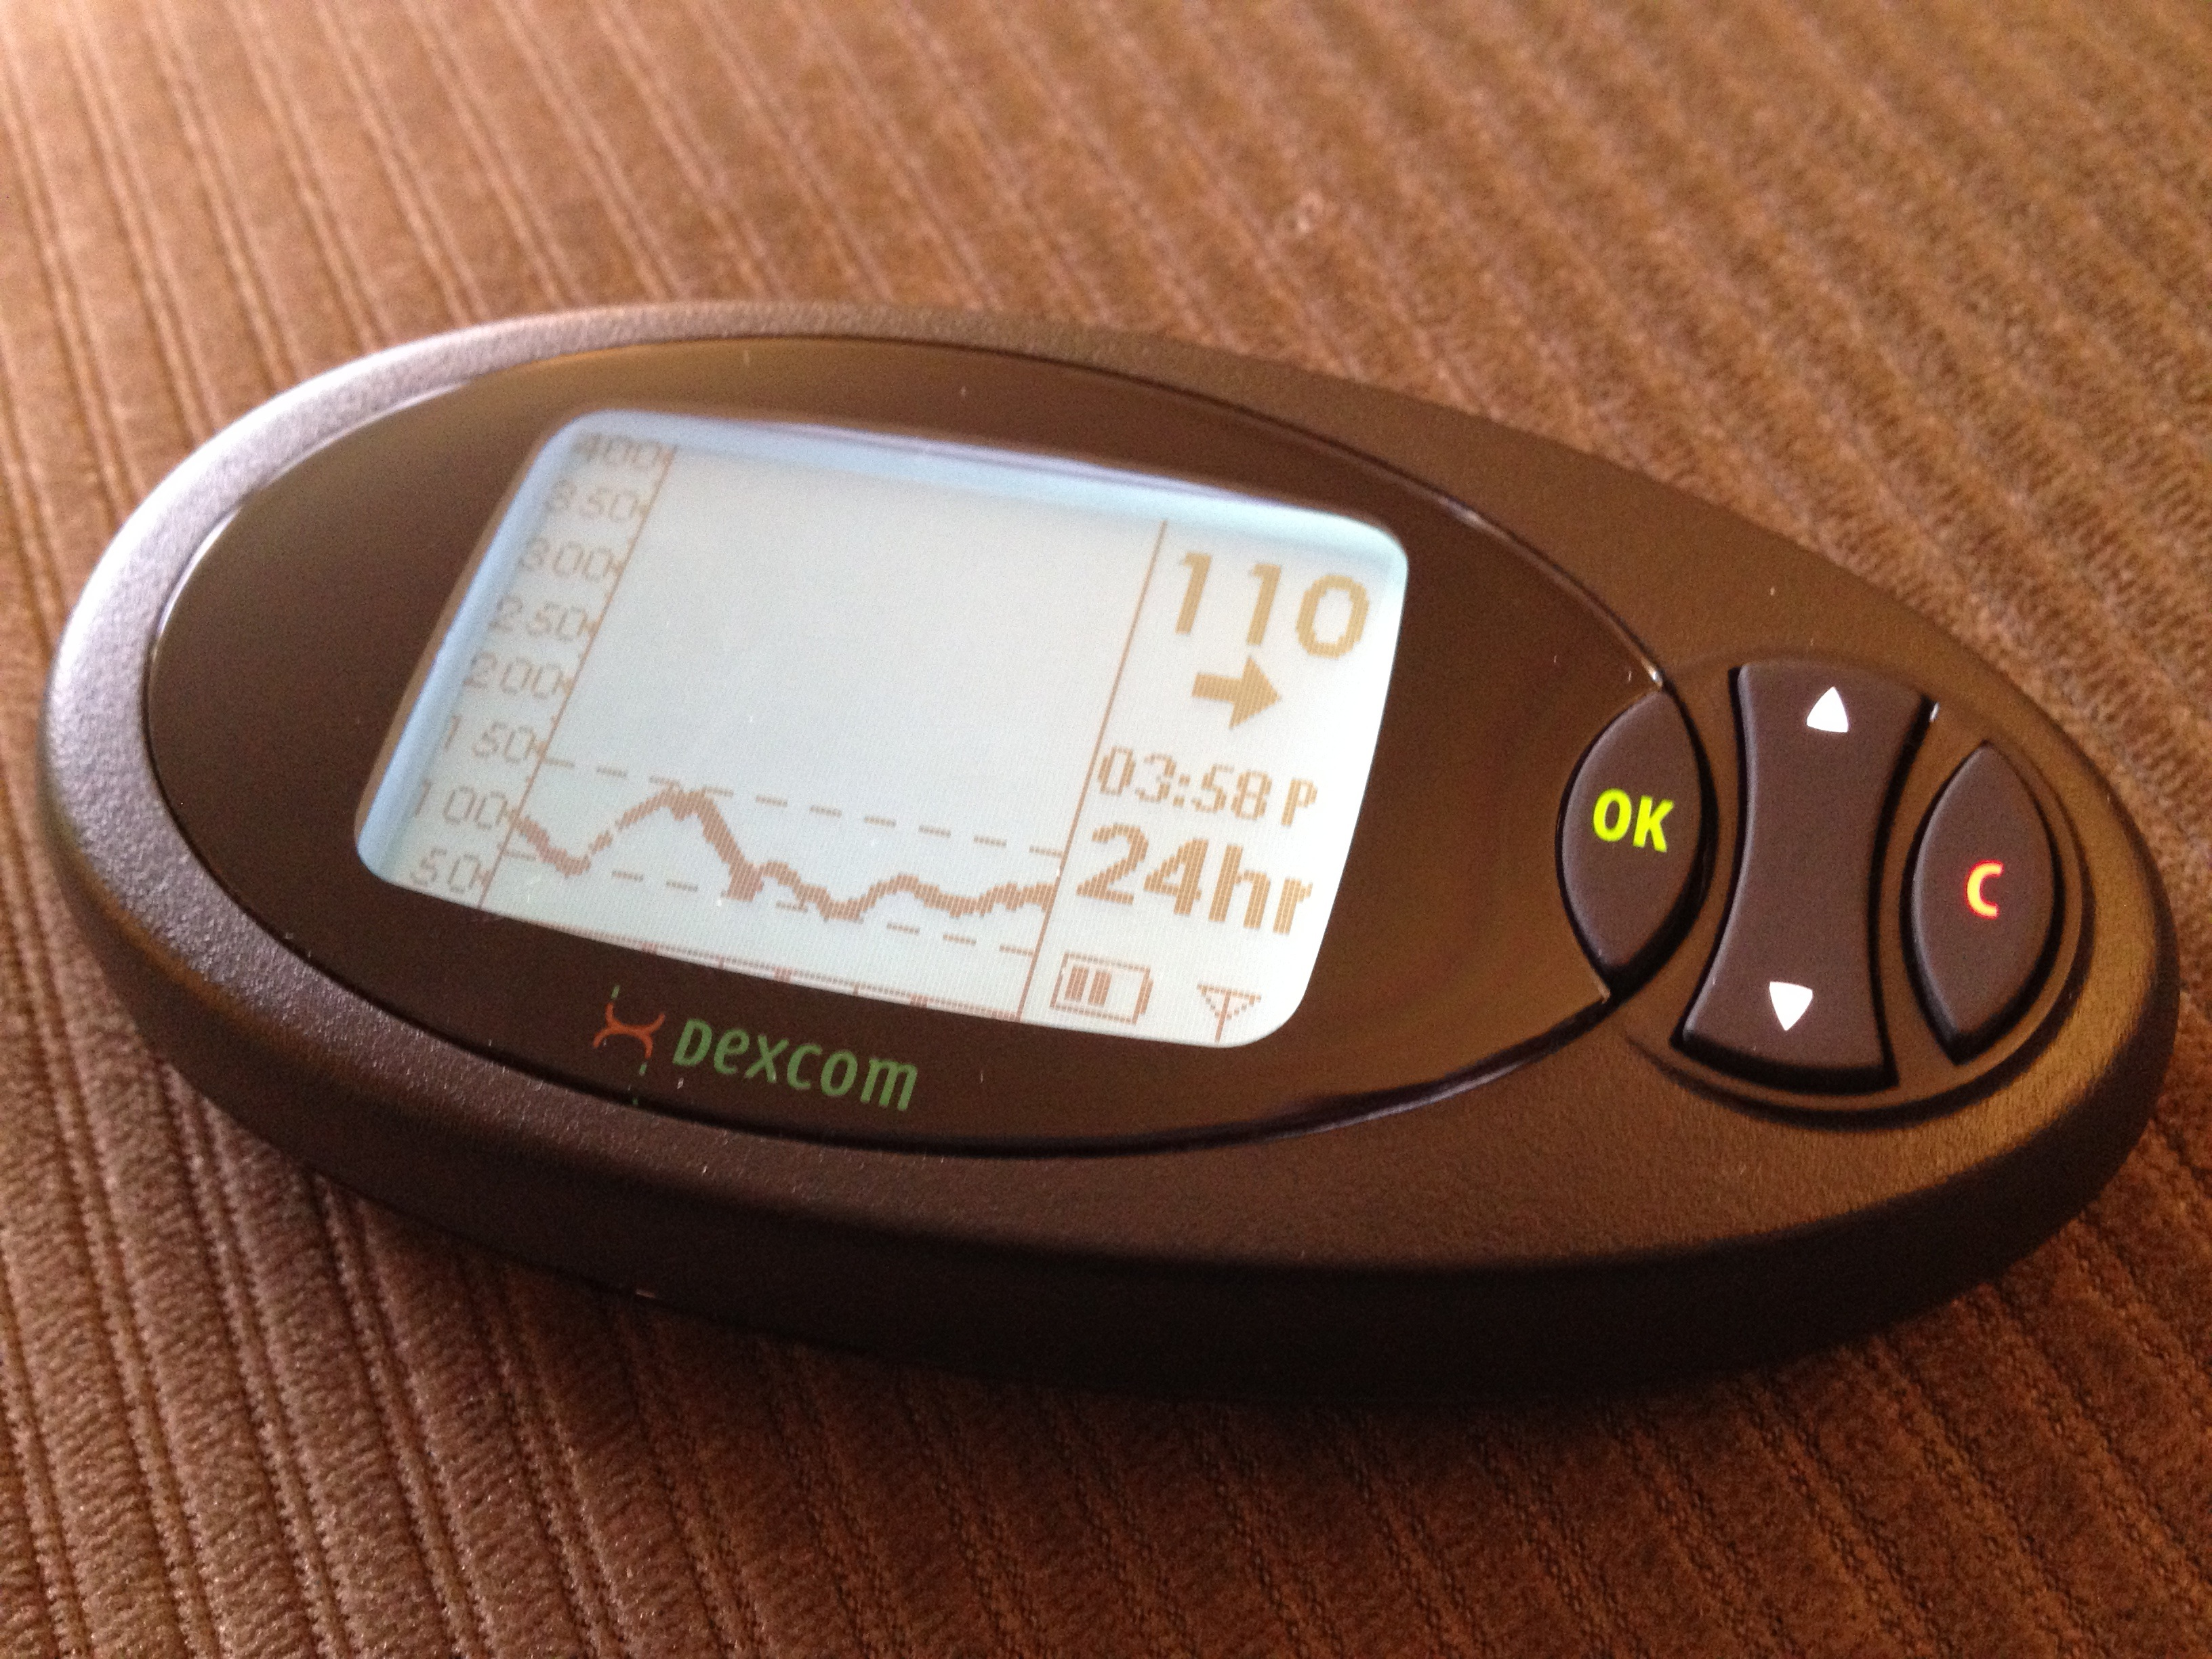
\includegraphics[width=.3\linewidth]{dexcom3.jpg}
      the Dexcom Continuous Glucose Monitor\\
      (Seven+ generation, now on G4 Platinum)
    \end{center}

\end{frame}

\begin{frame}
  \frametitle{About the Dexcom}

  The Dexcom provides:
    \begin{itemize}
    \item an (approximate) blood glucose reading every five minutes
    \item an arrow indicating
    \begin{itemize}
    \item trend (= up, down, or steady)
    \item rate-of-change
    \end{itemize}
    \item audible and/or vibrating alerts when blood glucose is
      \begin{itemize}
      \item too high
      \item too low
      \item or changing \textit{very} rapidly
      \end{itemize}
    \item ability to download data!
    \end{itemize}
\end{frame}

\begin{frame}
  \frametitle{Blood Glucose Management}

  \begin{itemize}
  \item non-diabetics blood glucose: between 70-130 mg/dL
  \item my goals:
    \begin{itemize}
    \item as many readings in the ``target'' non-diabetic range as possible
    \item keep the \% of readings \textit{below} 65 mg/dL to a minimum
    \item reduce standard deviation (as measured on a day's worth of readings)
    \item reduce mean
    \end{itemize}
  \end{itemize}

\end{frame}

\section{What I Did}

\begin{frame}
  \frametitle{My Experiment}

  \begin{itemize}
  \item first experience with Dexcom= \textit{shock}
  \item next= \textbf{frustration}
  \end{itemize}
  
\end{frame}

\begin{frame}
  \frametitle{My Experiment, Cont'd}

  \begin{hypothesis}
    Carbohydrate restriction is an effective way to improve blood glucose outcomes.
  \end{hypothesis}

\end{frame}

\begin{frame}
  \frametitle{Inspiration}

\href{http://www.amazon.com/Good-Calories-Bad-Challenging-Conventional/dp/1400040787}{\textit{Good Calories, Bad Calories} by Gary Taubes}\\
\vskip .5in

\begin{quote}
When I hear a physician saying to a type 1 diabetes patient, ``Go ahead and eat whatever you want, just make sure you cover your glucose with insulin,'' it's like telling a firefighter, ``Just go ahead and pour as much gasoline as you like on that fire you're trying to put out, as long as you cover it with enough water.''
\end{quote} \hskip .5in ---
\href{http://asweetlife.org/a-sweet-life-staff/featured/the-ketogenic-diet-and-peter-attias-war-on-insulin/24184/}{Dr. Peter Attia}
  
\end{frame}

\section{How I Did It}

\begin{frame}
  \frametitle{Tools}
  
  \begin{itemize}
  \item Dexcom data export formats:
    \begin{itemize}
    \item XML files, useful for manipulating in Python with \href{http://www.crummy.com/software/BeautifulSoup/}{BeautifulSoup}
    \item tab-delimited .csv files, useful for direct importing into R
    \end{itemize}
  \item in \href{http://www.r-project.org/}{R}:
    \begin{itemize}
    \item built-in non-parametric statistical functions
    \item built-in plotting functions: boxplot(), etc.
    \item \href{http://had.co.nz/ggplot2/}{ggplot2}
    \end{itemize}
  \end{itemize}
\end{frame}

\section{What I Learned}

\begin{frame}
  \frametitle{Visualizing Change: Violin Plot}

  \begin{center}
  2-month data samples from 2011 and carb-restriction experiment in 2012.
    \includegraphics[height=0.85\textheight]{../img/dexcom_violin_2month_samples.pdf}
  \end{center}

\end{frame}

\begin{frame}
  \frametitle{Comparing Years: Violin Plot}

  \begin{center}
  All of 2011 compared with all of 2012.
    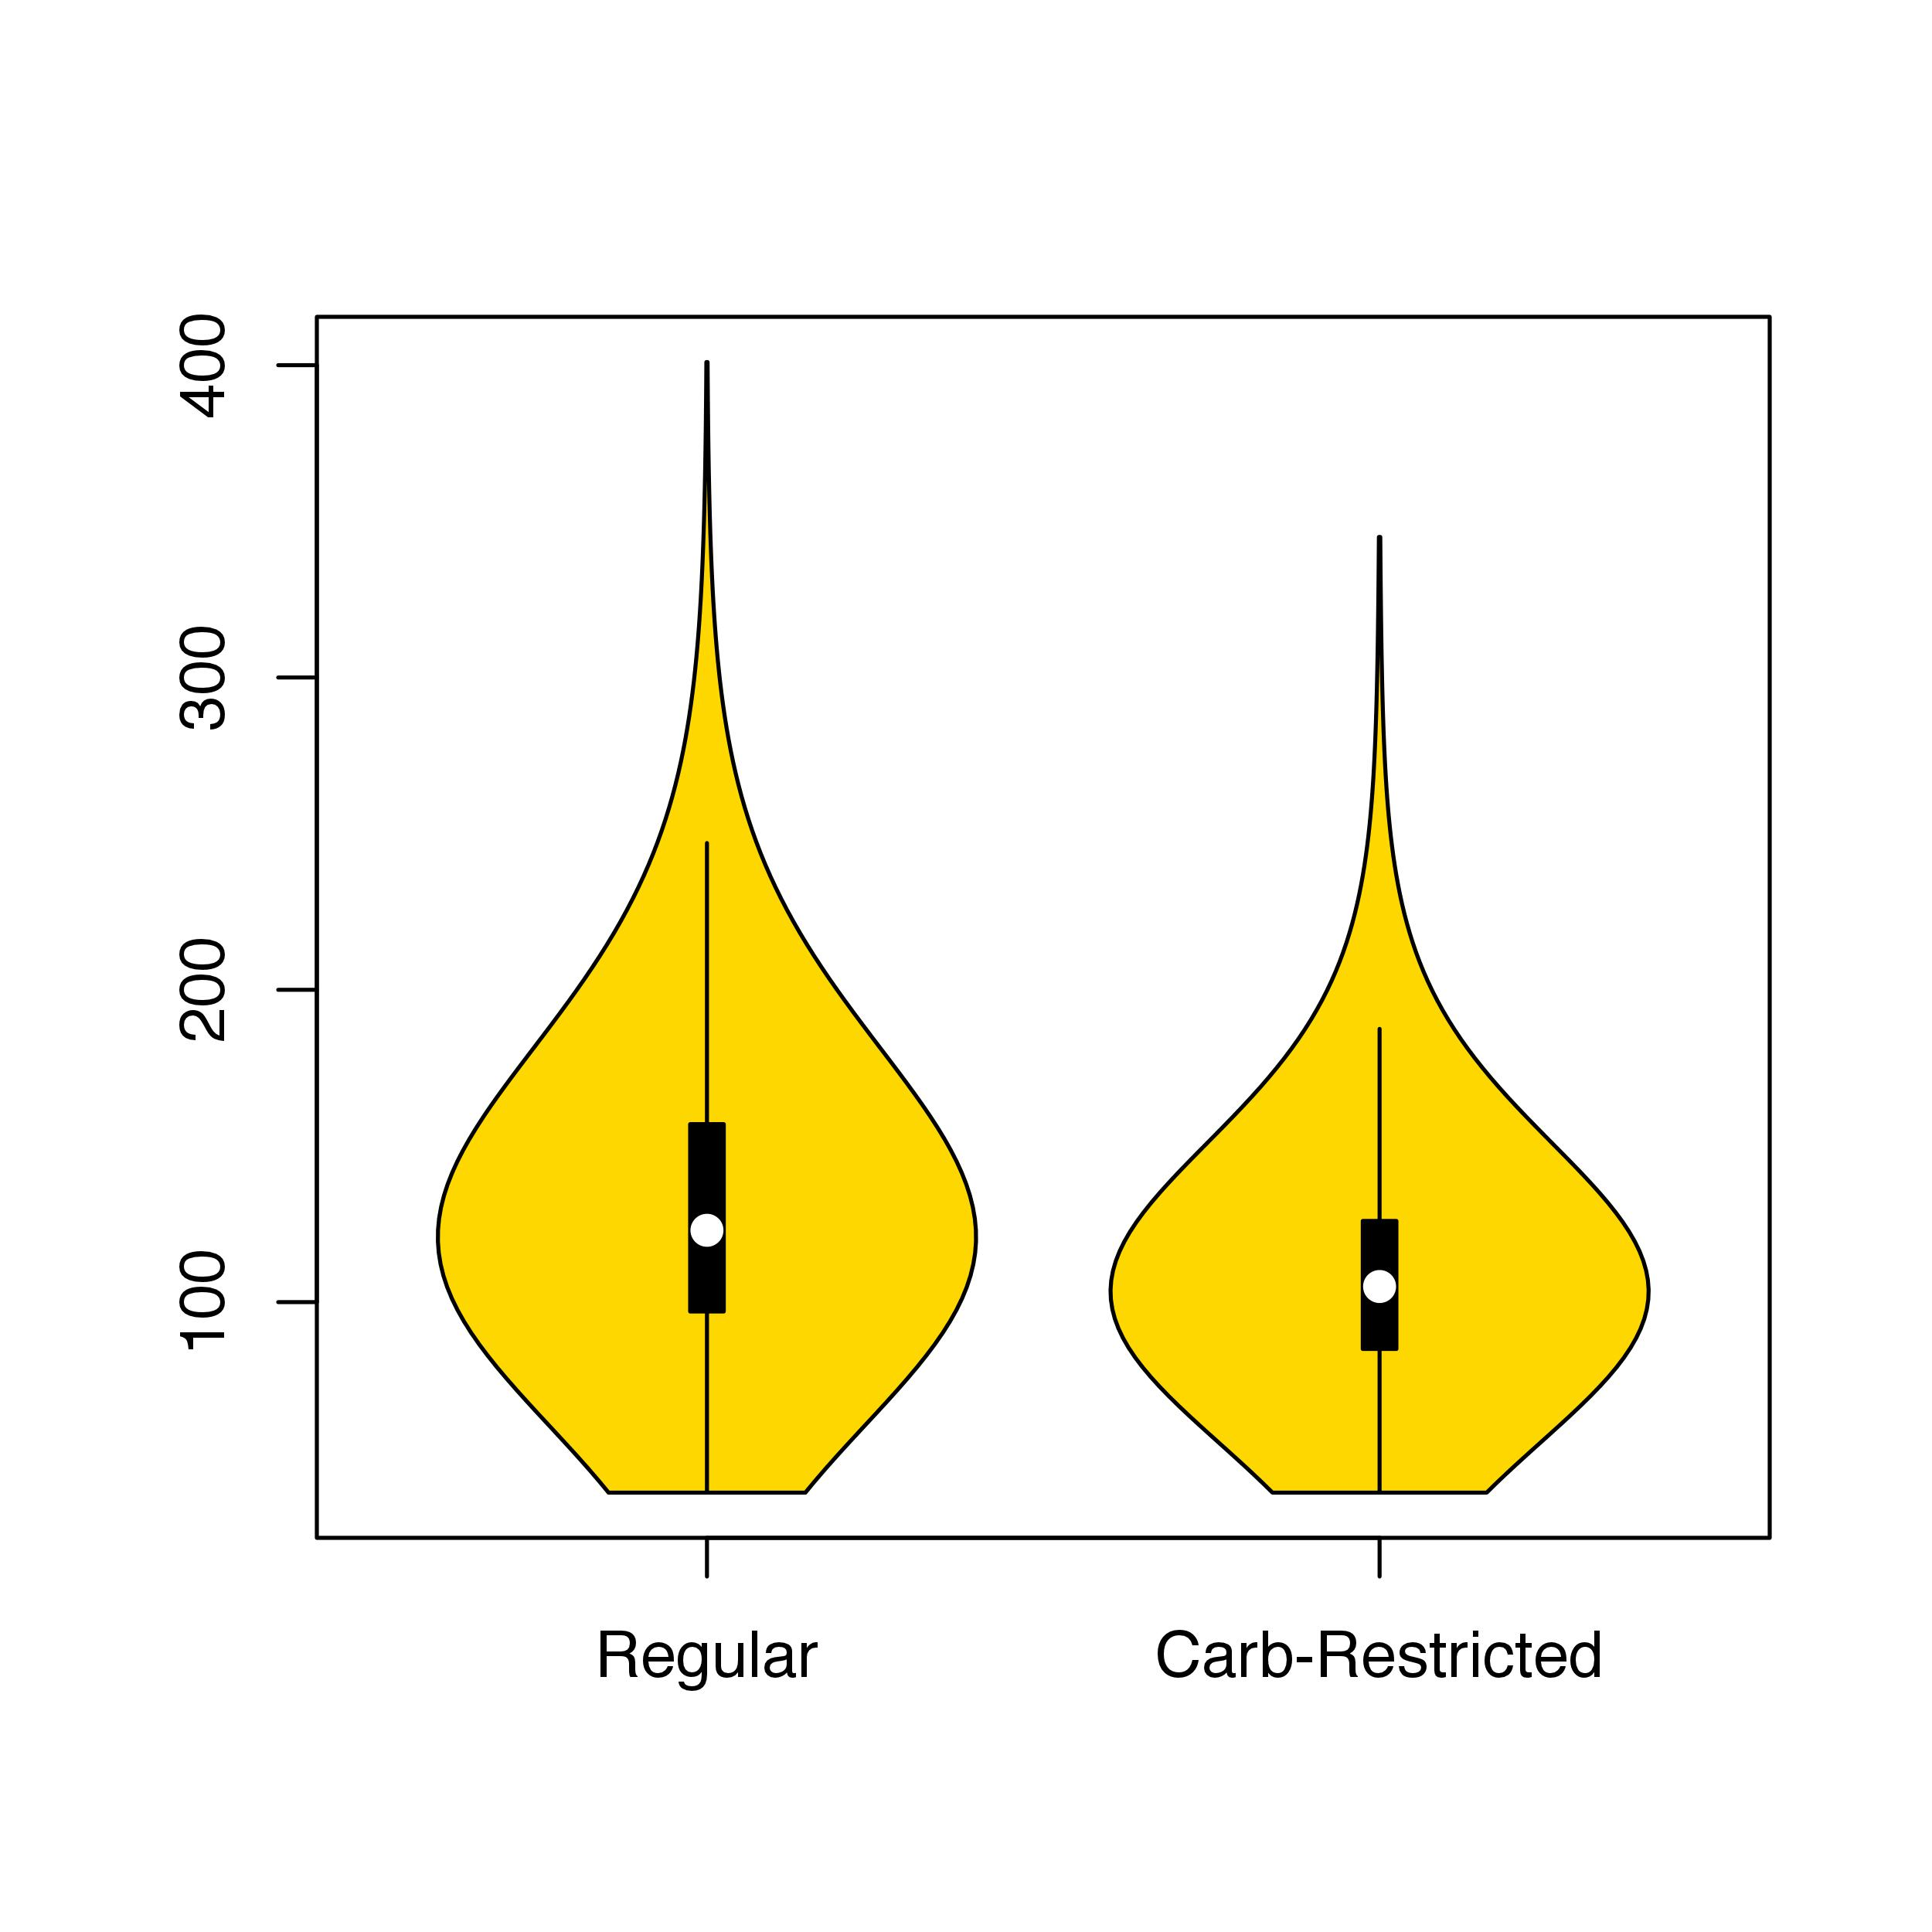
\includegraphics[height=0.85\textheight]{../img/dexcom_violin.pdf}
  \end{center}

\end{frame}

\begin{frame}
  \frametitle{Visualizing Change: Daily Mean over Time}

  \begin{center}
    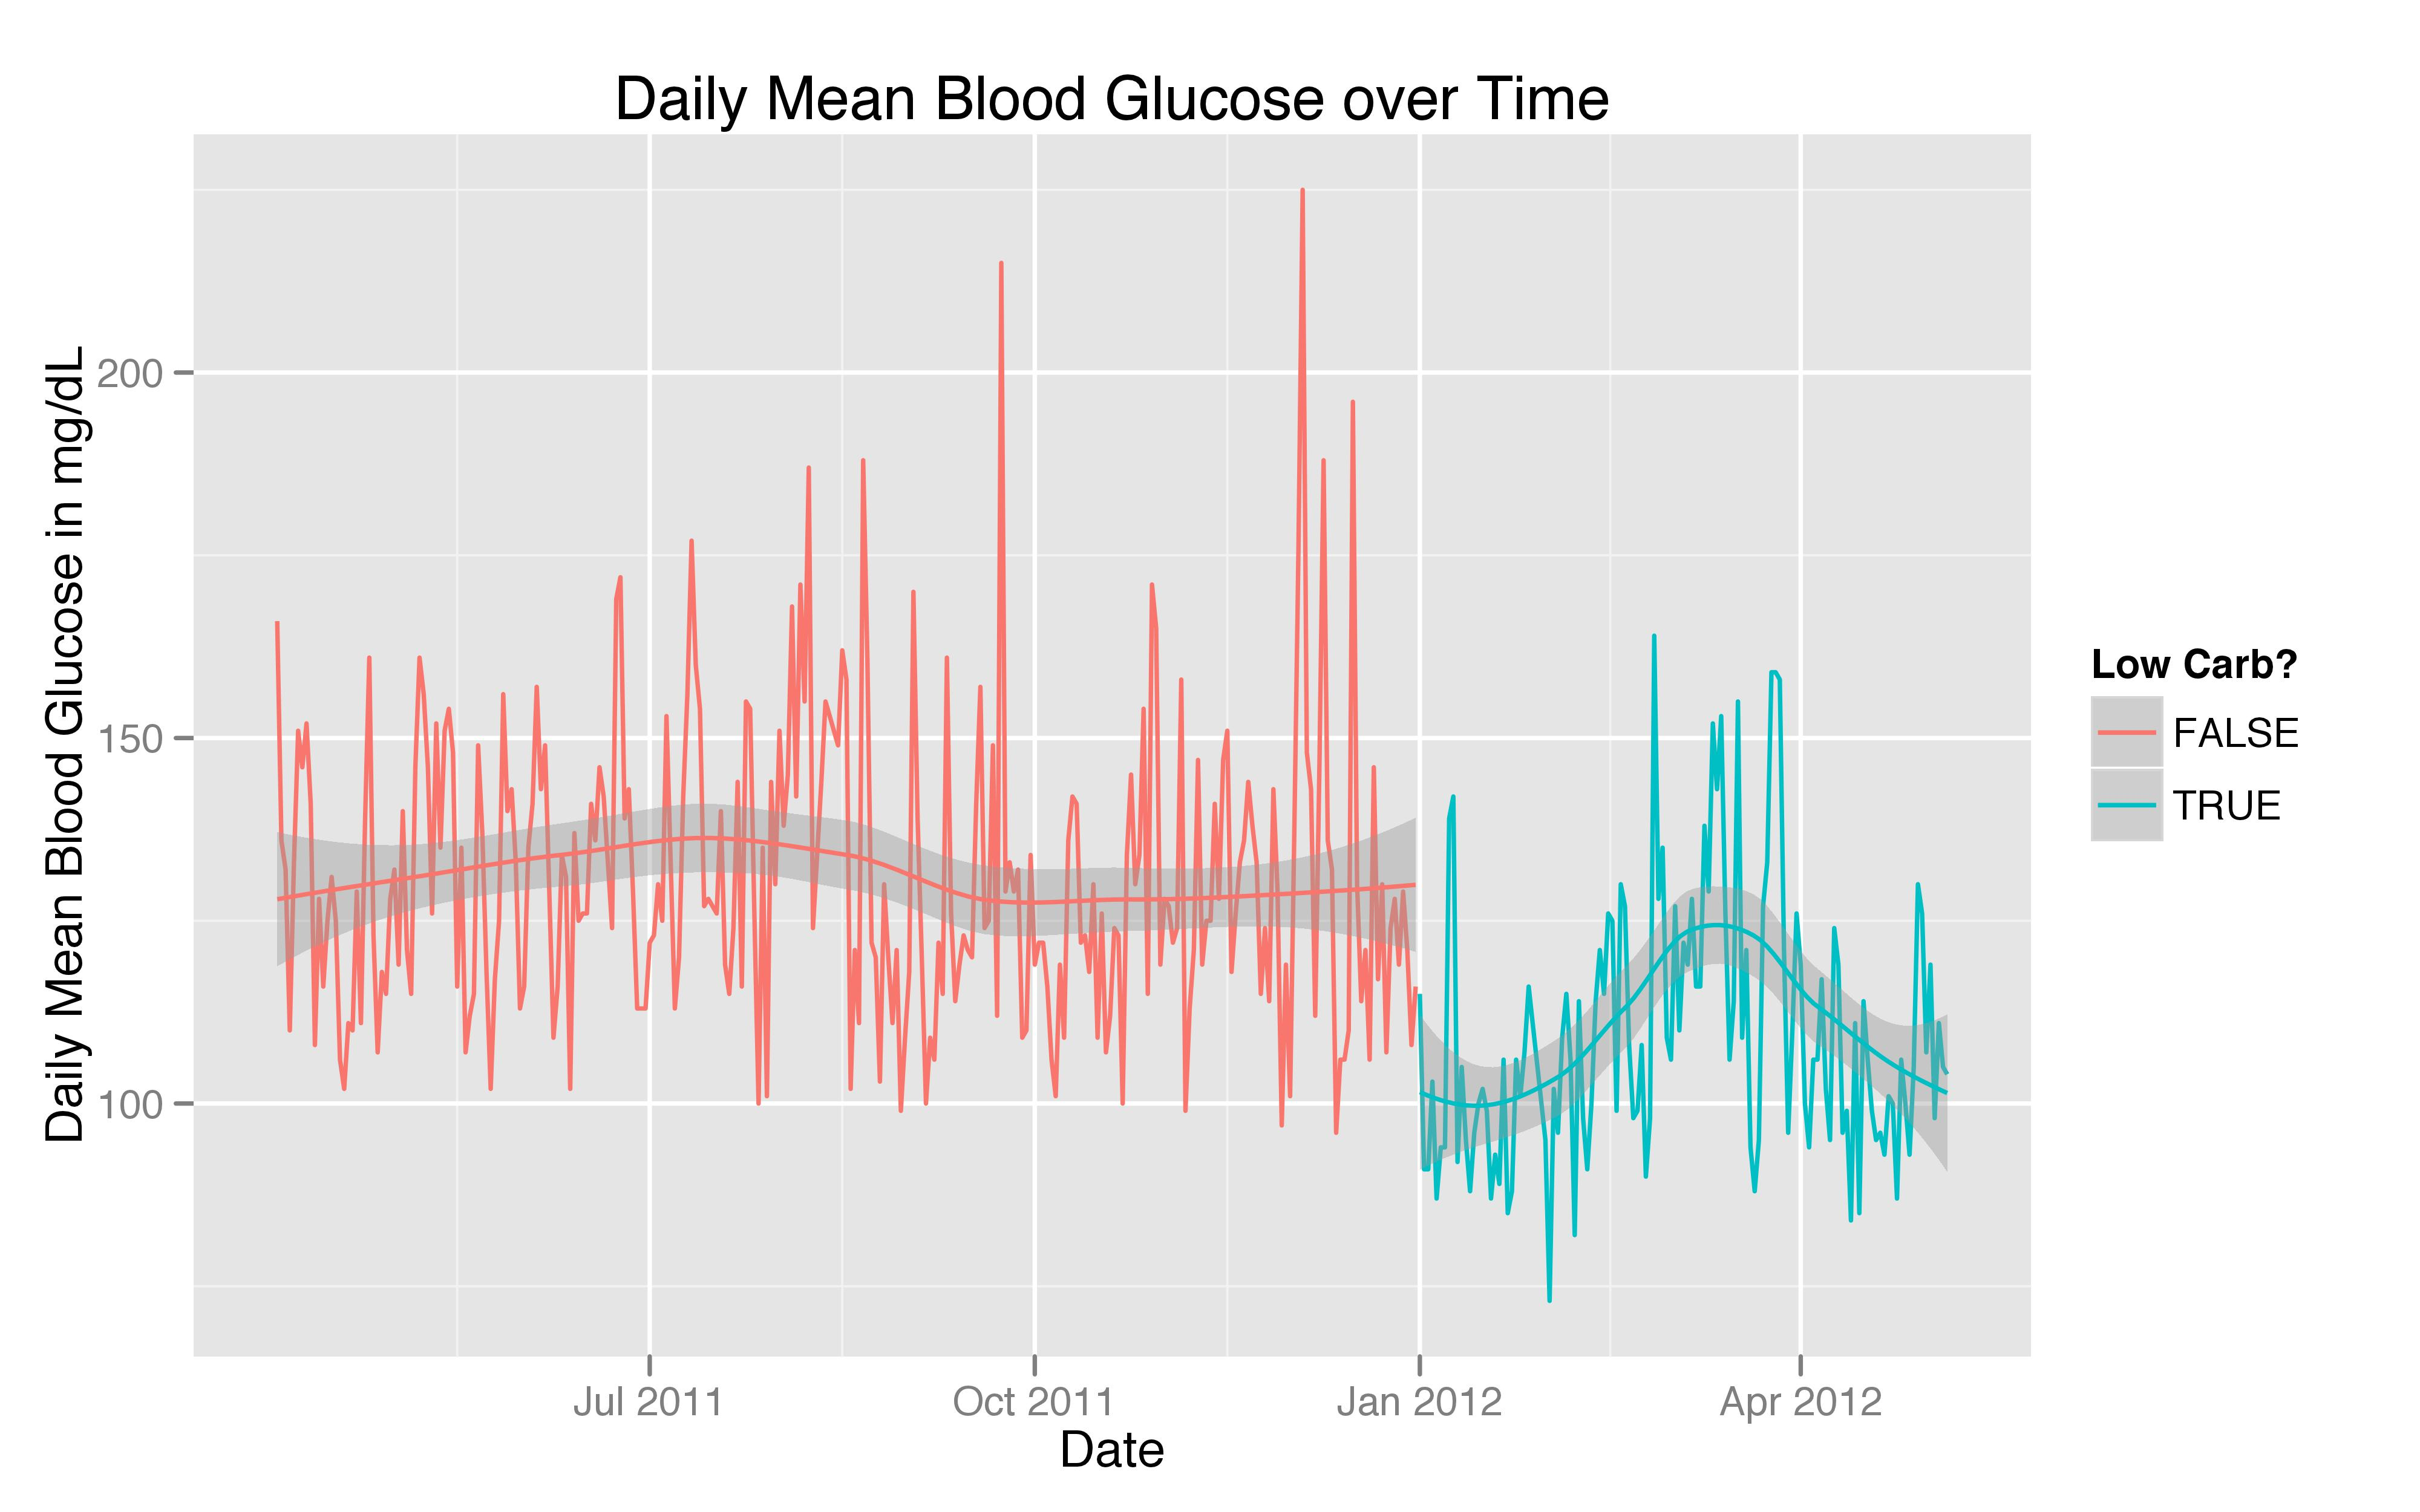
\includegraphics[width=\textwidth]{mean_blood_glucose.jpg}
  \end{center}

\end{frame}

\begin{frame}
  \frametitle{Visualizing Change: Daily Std. Deviation over Time}
  
  \begin{center}
    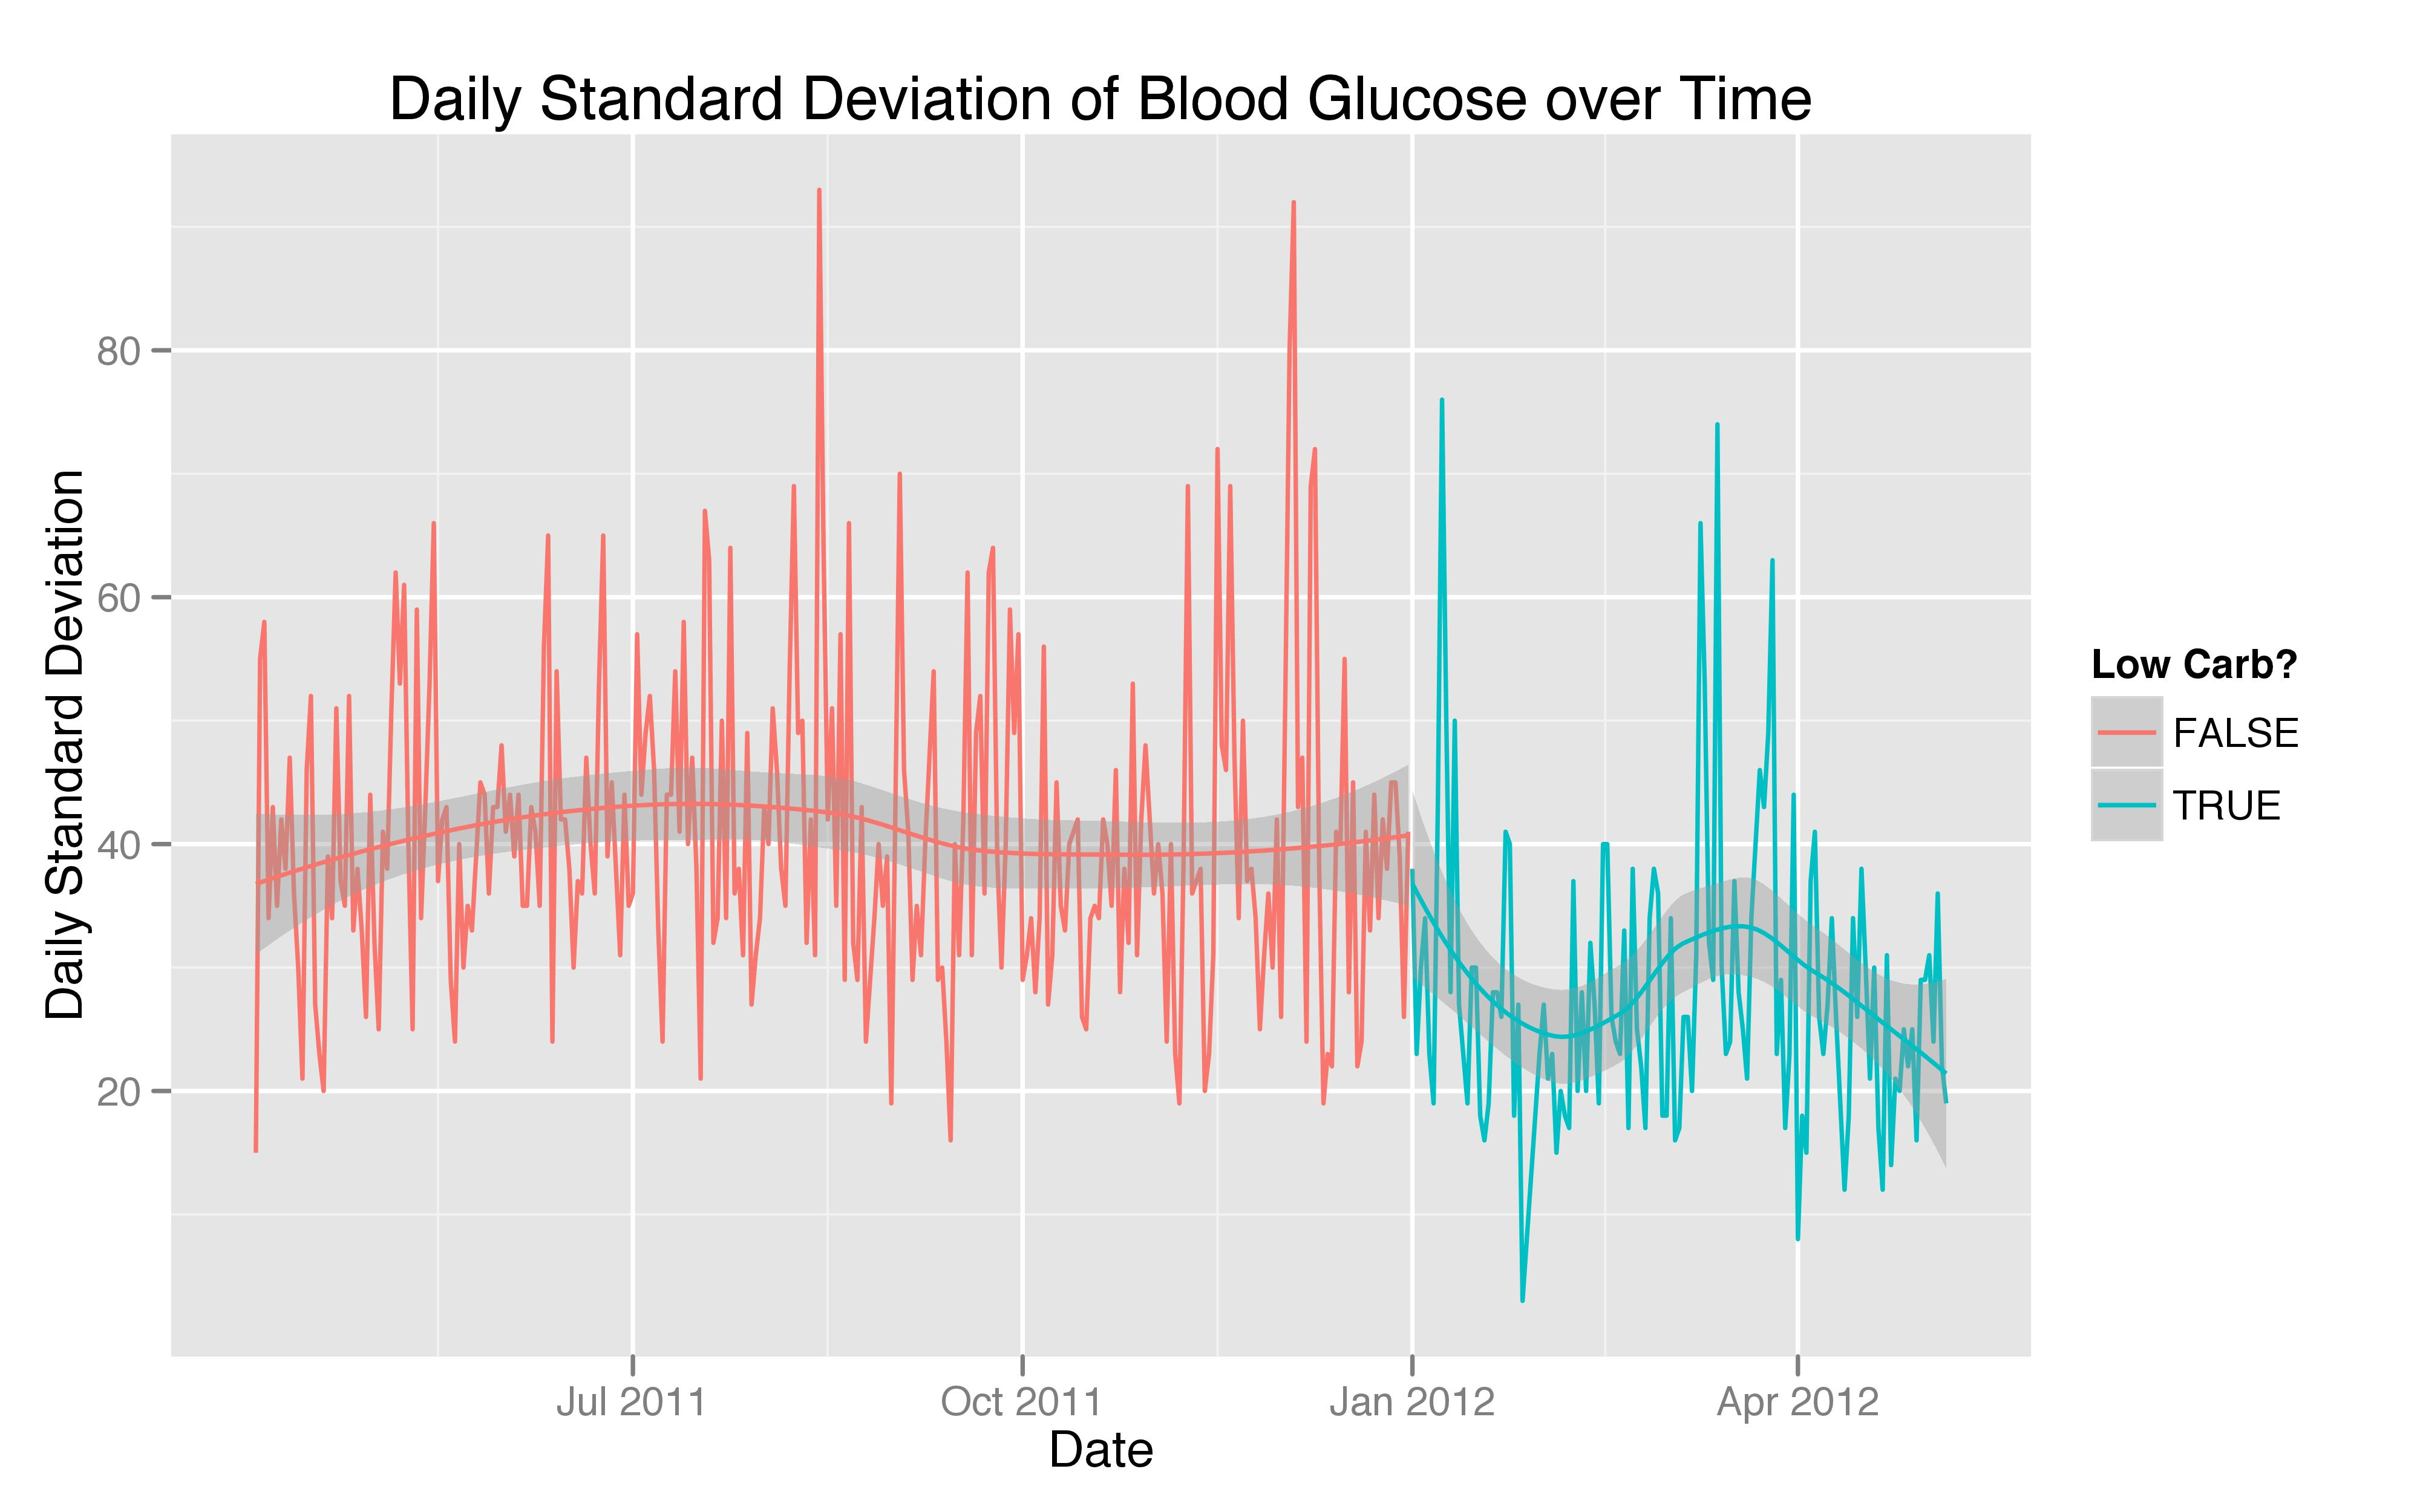
\includegraphics[width=\textwidth]{standard_deviation.jpg}
  \end{center}

\end{frame}

\begin{frame}
  \frametitle{Visualizing Change: Daily \% Low over Time}
  
  \begin{center}
    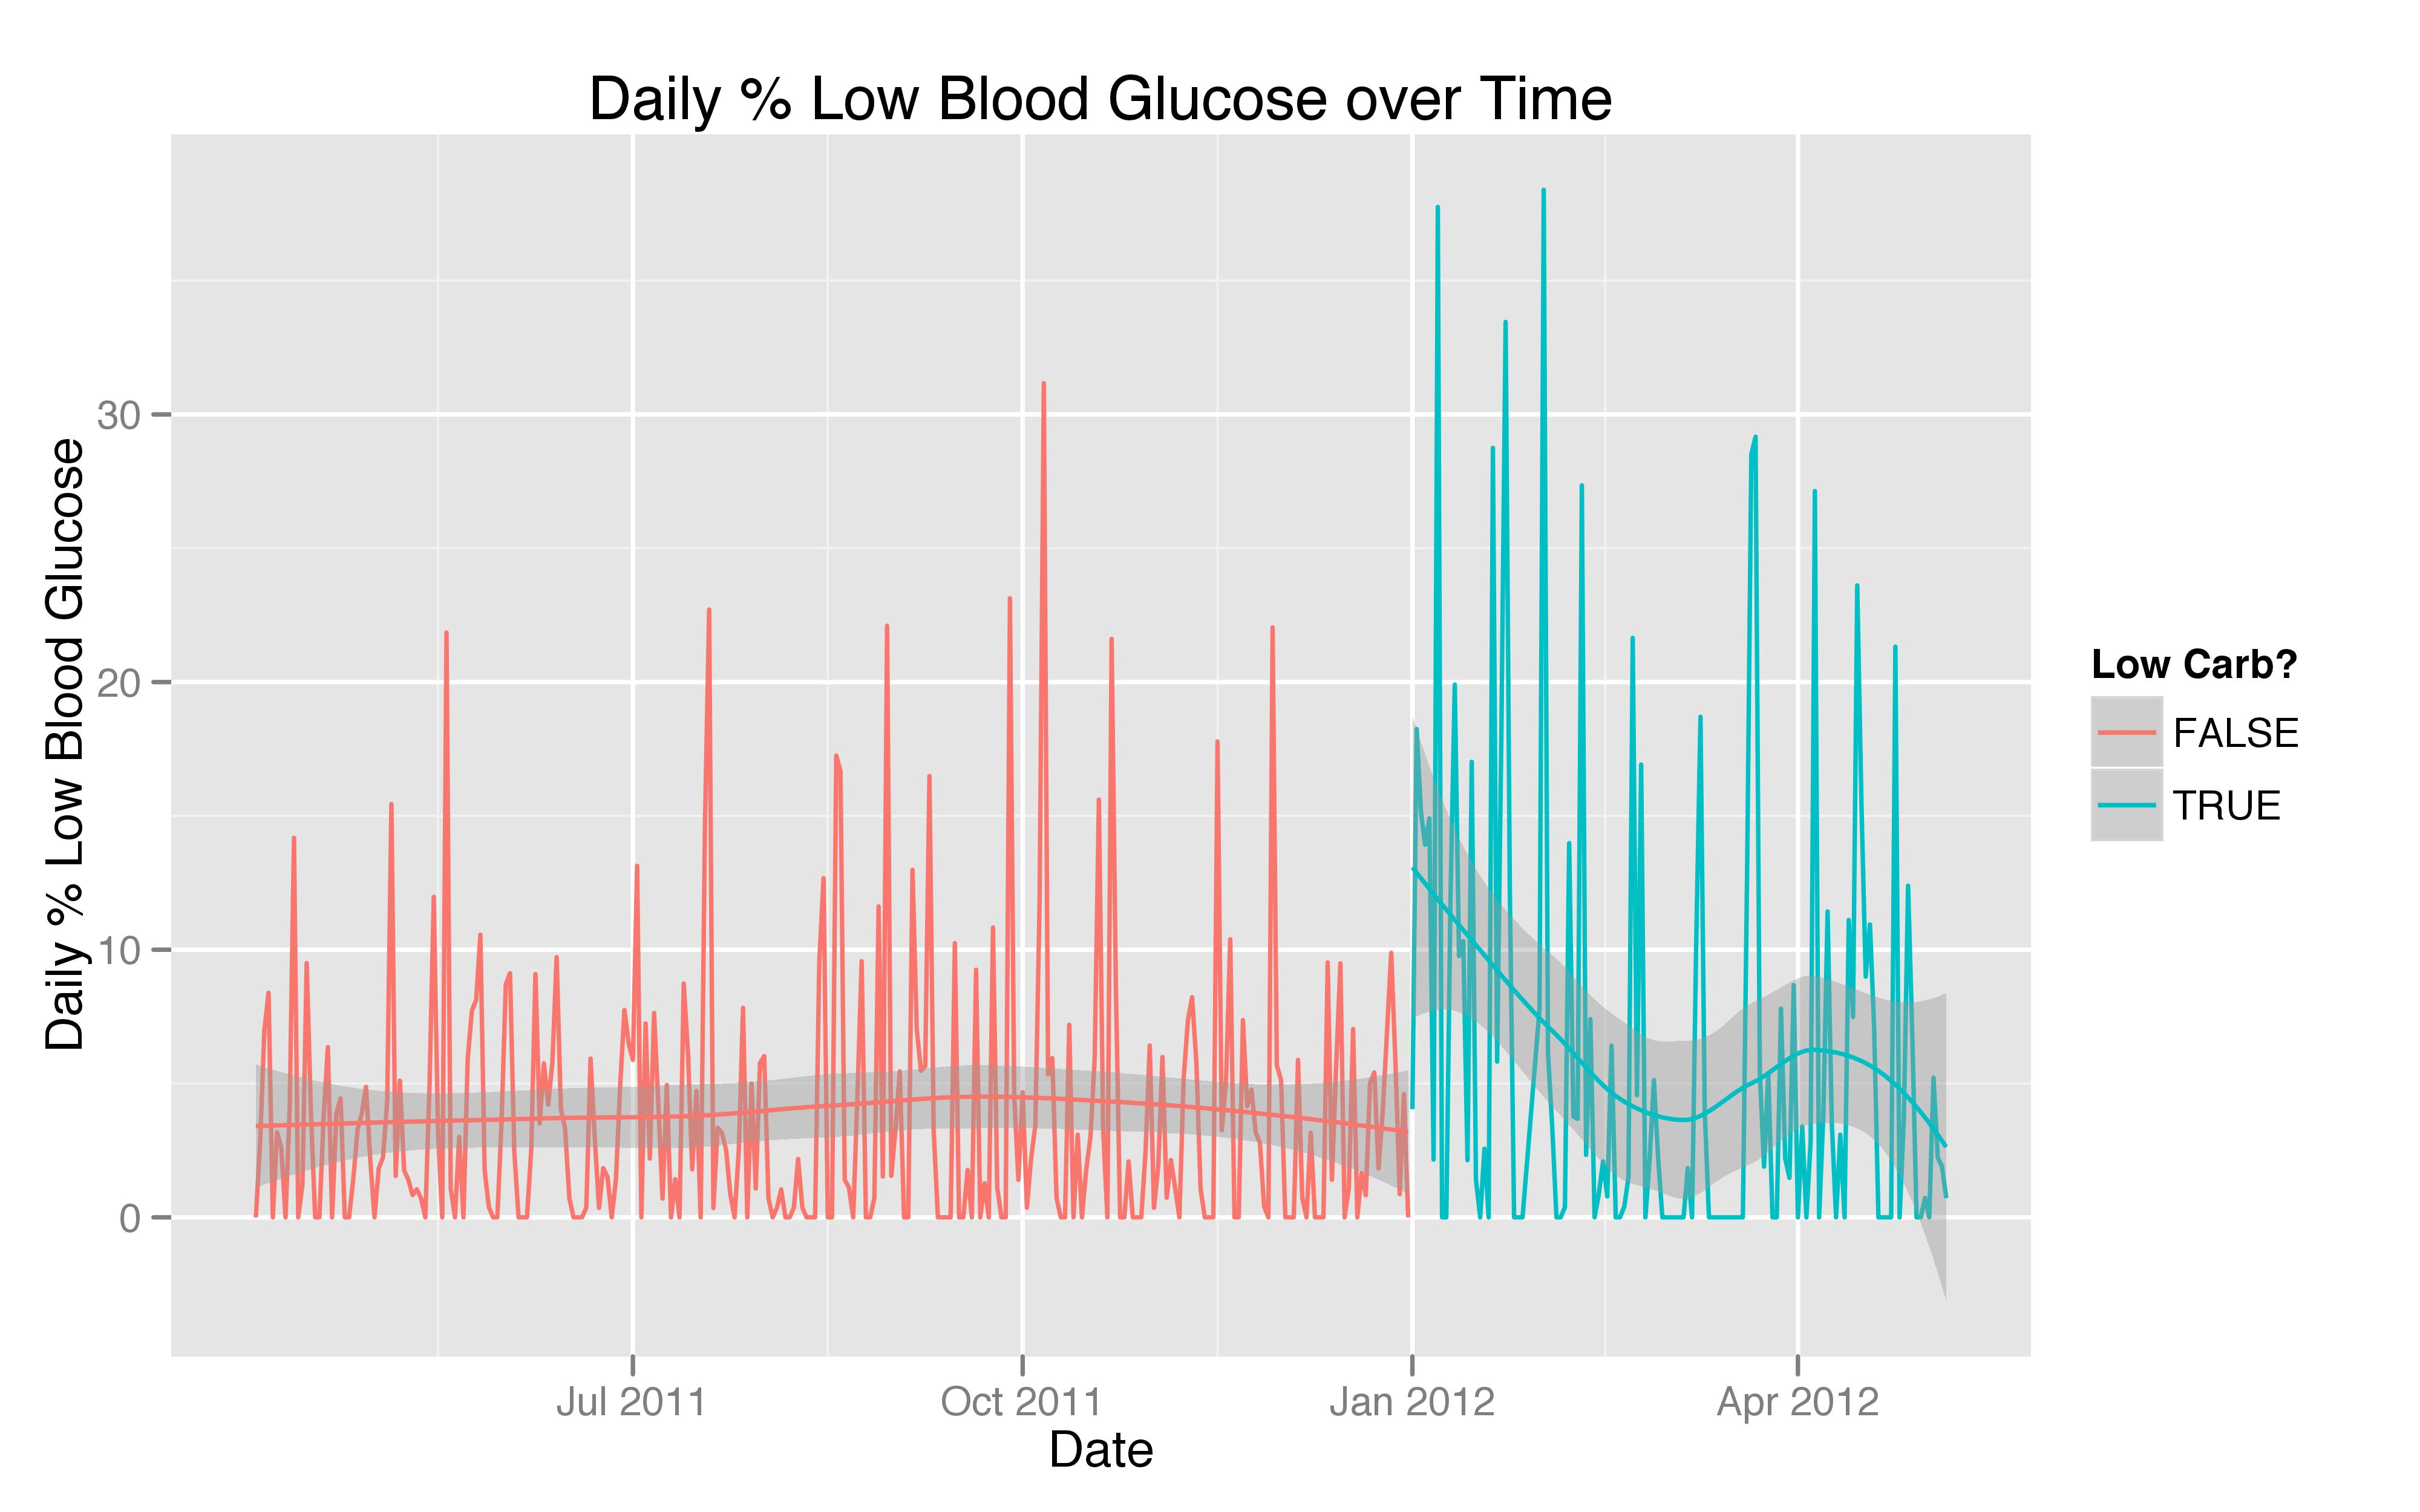
\includegraphics[width=\textwidth]{daily_low.jpg}
  \end{center}

\end{frame}

\begin{frame}
  \frametitle{Visualizing Change: Daily Percentages over Time}
  
  \begin{center}
    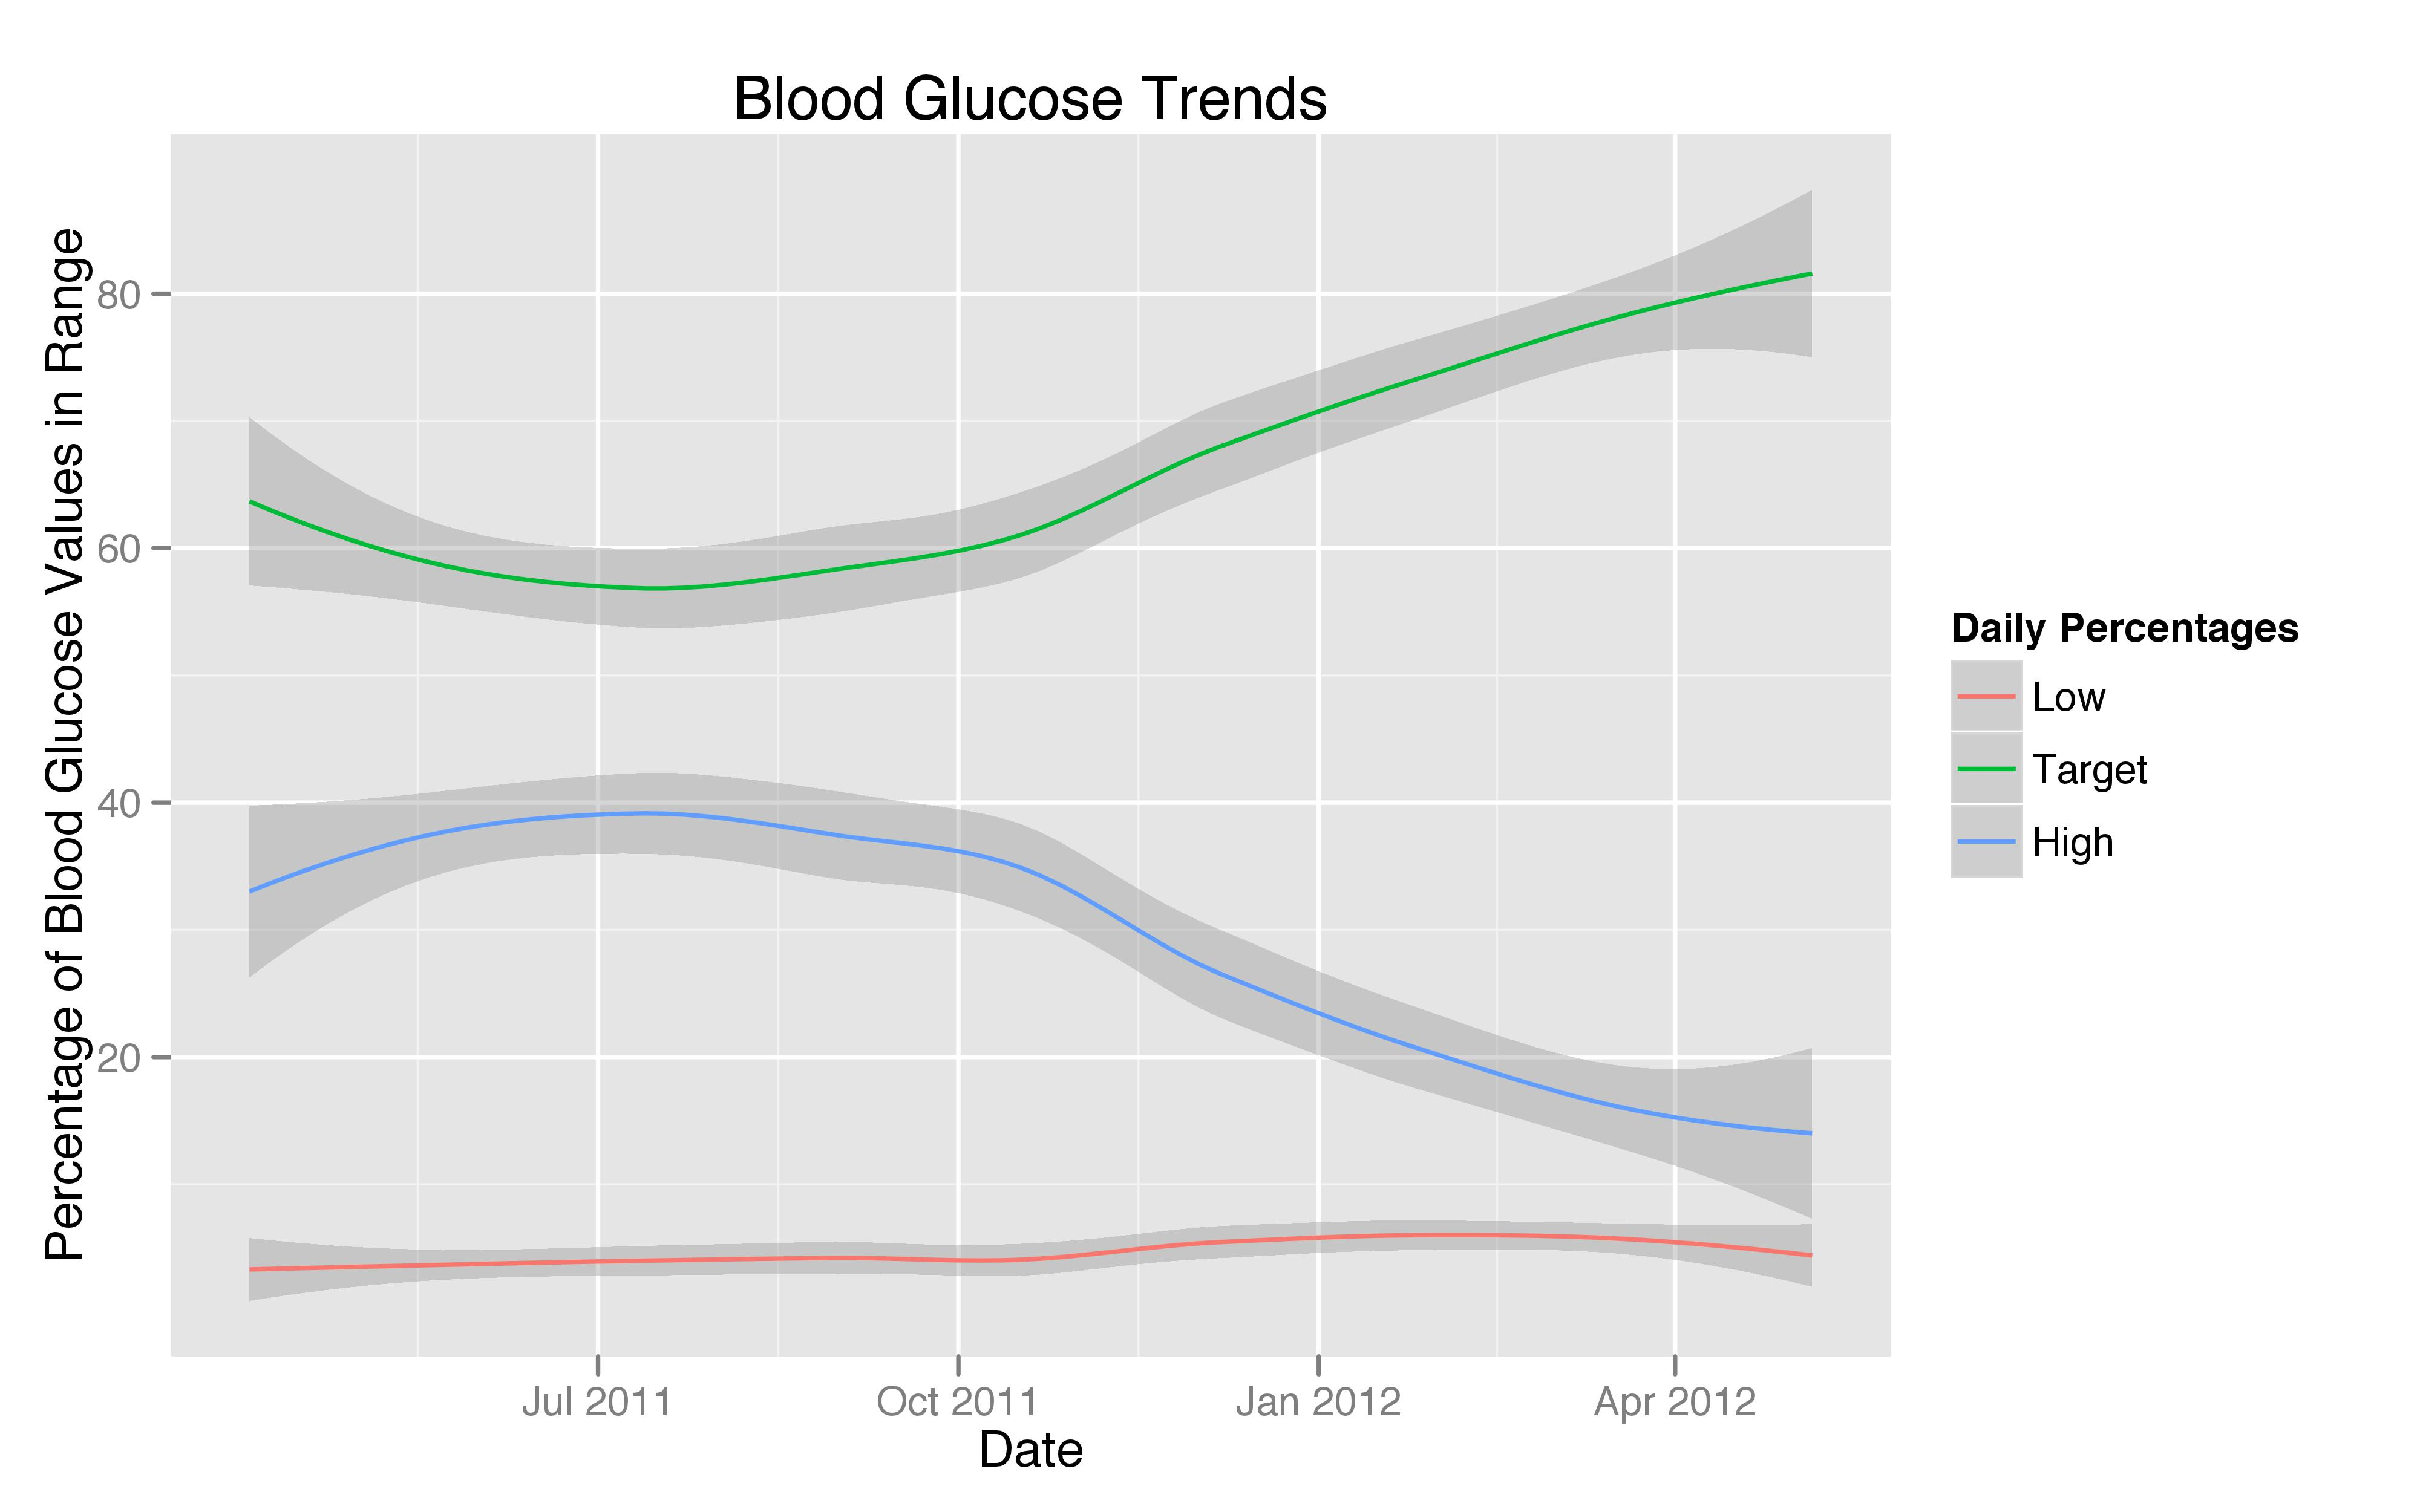
\includegraphics[width=\textwidth]{percentages.jpg}
  \end{center}

\end{frame}

\begin{frame}
  \frametitle{Statistical Significance}

  \begin{question}
     Did adopting a carbohydrate-restricted diet starting January 1st, 2012 result in a statistically significant difference in
     blood glucose?
  \end{question}
  Wilcoxon rank-sum test:
  \begin{itemize}
  \item similar to the Student's t-test, but for non-parametric (= non-normally-distributed) data
  \item \textbf{\texttt{p-value < 2.2e-16}}
  \item \textbf{Conclusion:} change in diet resulted in significant (negative) change in blood glucose values
  \item estimate of the median of the difference between a sample from regular diet blood glucose data and a sample from low-carb
    diet data is \textbf{about $-$19 mg/dL}
  \end{itemize}

\end{frame}

\begin{frame}
  \frametitle{Patterns: Time of Day}
  
  \begin{center}
    \includegraphics[height=0.9\textheight]{../img/hour_heatmap.pdf}
  \end{center}
\end{frame}

\begin{frame}
  \frametitle{Thanks!}

  Contact: \href{jana.eliz.beck@gmail.com}{\texttt{jana.eliz.beck@gmail.com}}\\

  \vskip .5in

  Upcoming Project: \href{https://github.com/jebeck/iPancreas}{\texttt{https://github.com/jebeck/iPancreas}}\\

  \vskip .1in

  \small{(Description here: \href{http://jebeck.github.com/iPancreas/}{\texttt{http://jebeck.github.com/iPancreas/}})}

\end{frame}

\end{document}